\section{Introduction}
In this computer based test we are asked to perform linear regression by least squares on a given data set. The dataset analysed is the Olympic men's running time (100m and 400m) for a range of years. 

This report will outline the findings and elaborate on certain pieces of code, which are shown in the listings. Refer to the appendices for a listing of the complete code for Tasks 1 and 2.
\section{Task 1}
In Task 1, we are asked to load and analyse the Olympics men's 400m data. We then have to fit the \textbf{n} order polynomial functions to this data, where \textbf{n} is 1 to 4, and use 10-fold cross-validation to choose the "best" value of \textbf{n}. In order to determine the "best" value of n, first we must define what is the best model. 

Insert something about regularisation and over fitting\\
Insert something about ability to accurately predict beyond training examples.

Insert summary of first task.\\
In short, first we determine the mean squared loss, \textbf{msl}, for each order \textbf{n}, and where loss is the difference between predicted and observed labels. We then plot \textbf{msl} against order \textbf{n}. Whilst, you can 

\begin{figure}[h]
	\centering
	\includegraphics[width=0.7\linewidth]{images/CVLossANDTrainLoss8}
	\caption{Comparison of the CV and Train loss plots}
	\label{fig:CVT8}
\end{figure}


In \ref{fig:CVT8}, we can see blah blah interpret graph, CV loss and Train loss, min point of both, decreases then increases

\begin{figure}[h]
	\centering
	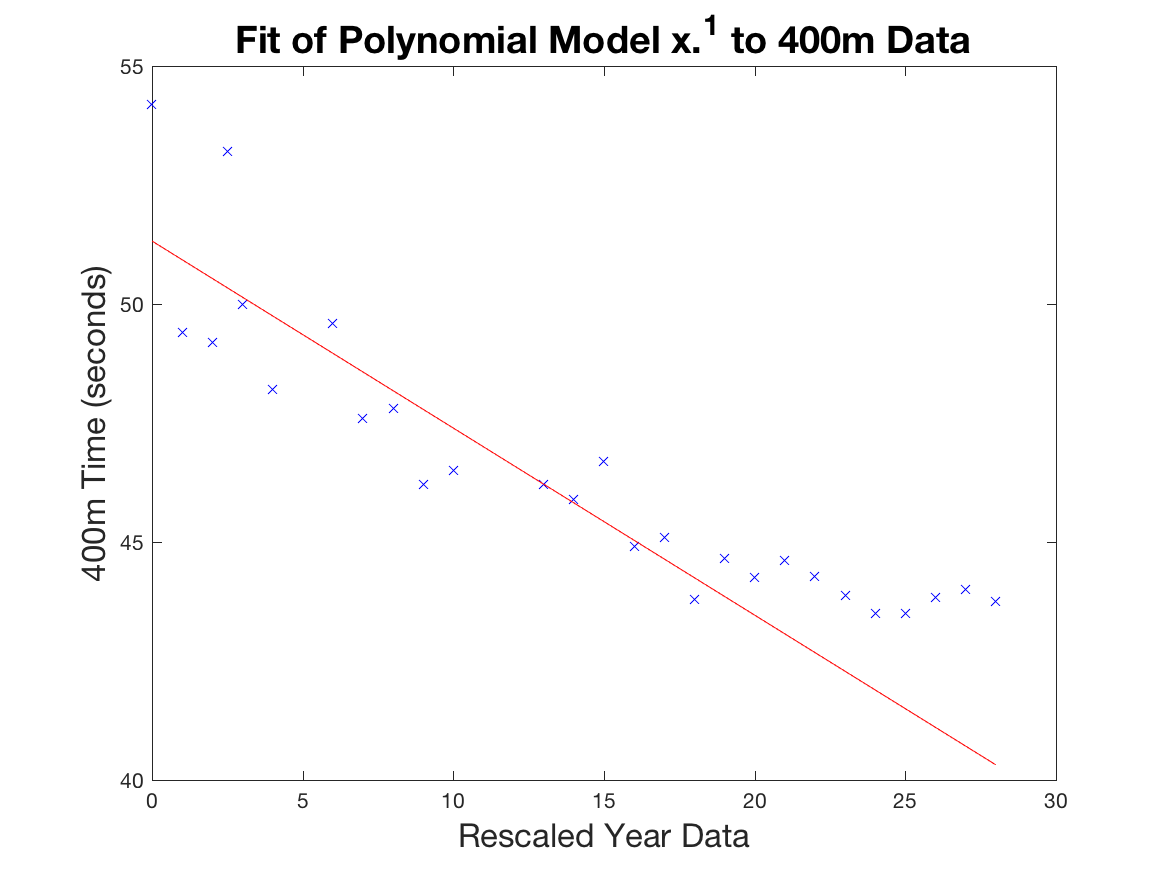
\includegraphics[width=0.7\linewidth]{images/model1}
	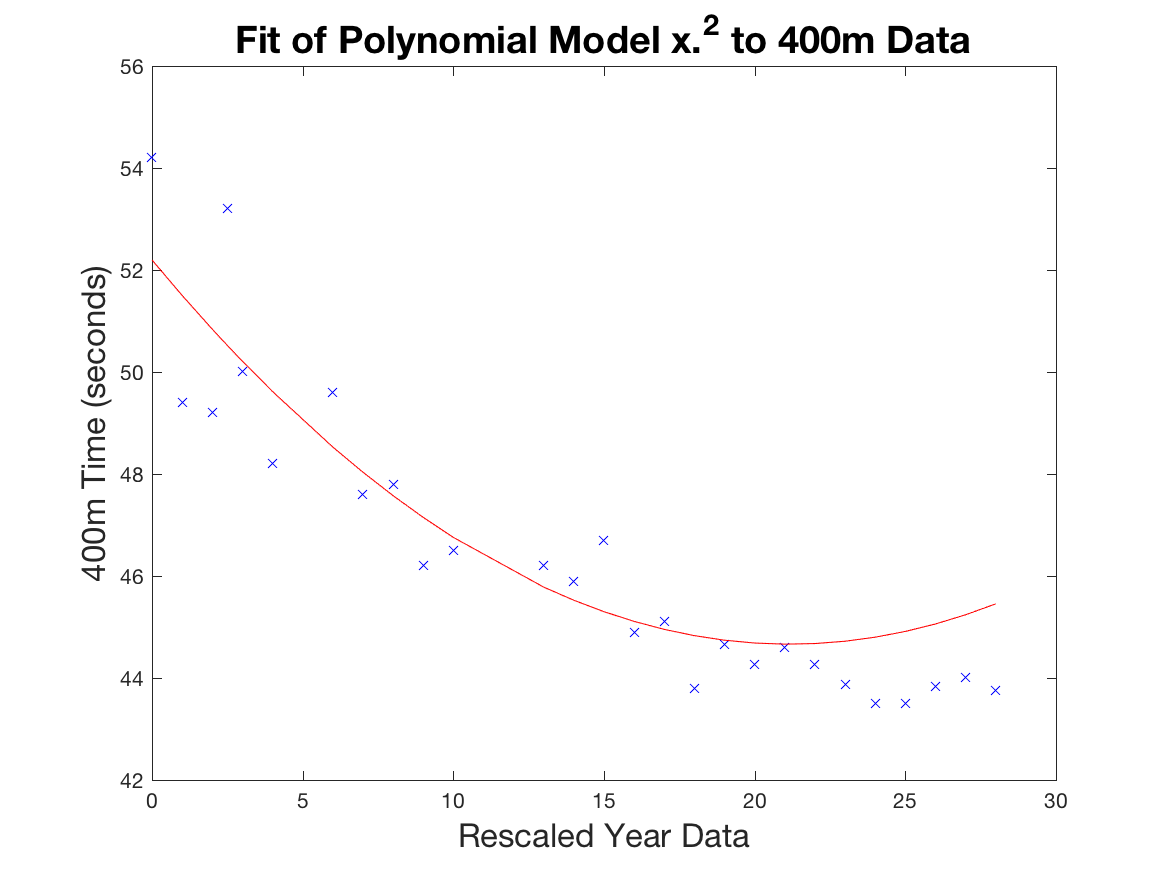
\includegraphics[width=0.7\linewidth]{images/model2}
	\caption{Polynomial functions with order 1 and 2}
	\label{fig:model1}
\end{figure}


TEXT: interpret and compare graphs

PIC: 3 and 4 order

Text: interpret and compare graphs

PIC: 27 order CV and train

TEXT: further insight; for a data set with m attributes, is fit perfectly by m-1 order. \\
Also, if we do not normalise data, we run into numerical errors when the polynomial function of the data.
\section{Task 2}
In task 2 we are given the task to find the value of $\lambda$ that gives the 'best' predictive performance on the Olympic men's 100m data using 5-fold cross-validation.
